\documentclass[11pt]{article}
\usepackage[backend=biber, sorting=none]{biblatex}
\usepackage{hyperref}
\usepackage{bbding}
\usepackage{graphicx}
\usepackage{booktabs}
\usepackage{multirow}
\usepackage[section]{placeins}
\usepackage{makecell}
\usepackage[title]{appendix}
\usepackage{subcaption}
\usepackage{float}
\usepackage{siunitx}
\usepackage{array}
\usepackage{tabularx}
\usepackage{theme}
\usepackage{shortcuts}
\usepackage{stmaryrd}
\usepackage{booktabs}
\usepackage[figurename=Fig.,font=small,labelfont=bf,labelsep=space]{caption}
\addbibresource{references.bib}

\title{XAI Project - MVA 2025/2026\\Diffusion Models for
Counterfactual Explanations:\\an Application to audio}
\author{
  Armand Blin \email{armand.blin@epita.fr} \\
  Romain Cargnello \email{romain.cargnello1@gmail.com} \\ % student 1
  Simon Sassi \email{sassisimon84@gmail.com} % student 2
}

\setcounter{page}{0}

\begin{document}
\maketitle
\thispagestyle{empty}
\tableofcontents

\newpage
%\pagestyle{plain}

\section{Introduction}

Deep neural networks have achieved remarkable success across a wide
variety of machine learning tasks, but their "black-box" nature
remains a main problem for human trust in their outputs. As these
models are increasingly deployed in real-world scenarios, the field
of Explainable AI (XAI) has emerged to help humans understand the
reasoning behind their decisions. Among the various XAI methods,
counterfactual explanations are particularly intuitive. Rather than
highlighting which features led to a specific decision, a
counterfactual explanation answers the question: \textit{"What
  minimal changes must be made to the input for the model to change its
prediction?"}

Recently, the \underline{Di}ffusion \underline{M}odels for
Counterfactual \underline{E}xplanations (DiME) framework
\cite{jeanneret2022diffusion} uses the state-of-the-art generative
power of diffusion models to produce high-fidelity counterfactuals.
By performing a partial classifier-guided diffusion, DiME
successfully generates high-fidelity counterfactuals for facial
attributes, ensuring a given image changes class while remaining
perceptually close to the original input.

However, while XAI techniques have been widely studied in the field
of computer vision (such as facial image processing), their
application to the audio domain remains relatively unexplored. Audio
signals have fundamentally different structural, temporal, and
frequency dynamics compared to natural images, making the generation
of coherent and realistic audio counterfactuals a unique and complex
challenge. In this project, we aim to bridge this modality gap by
adapting DiME to audio analysis, specifically focusing on
multi-instrument recognition.

By converting 1D audio waveforms into 2D mel spectrograms, we
maintain the core architecture of the DiME pipeline while addressing
the unique specificities of the audio domain. This modality
transition need significant changes, as the original dataset, the
pre-trained diffusion model and the guidance classifier.

\section{Diffusion Models for Counterfactual Explanations}

\underline{Di}ffusion \underline{M}odels for Counterfactual
\underline{E}xplanations (DiME) \cite{jeanneret2022diffusion} takes
advantage of the natural image generation power of diffusion models
to produce counterfactual explanations for face images. Its objective
is to invert a specific attribute in an initial image (for example
changing a smiling face to a non-smiling one) while preserving the
original image's characteristics as much as possible. First, we will
introduce relevant notions about diffusion models, before detailing
the mechanism behind DiME.

\subsection{Diffusion models in a nutshell}

Diffusion models are a recent class of generative models that rely on
two Markov chain sampling schemes that are inverses of one another.
The basic idea is simple: by learning how images are progressively
corrupted by noise in a forward pass, the model can reverse this
process to generate new, natural images from pure noise.

\paragraph{The forward process}

The forward process starts from a clean natural image $x_0 \sim p(x)$
and iteratively samples $x_1, \dots, x_T$ by progressively replacing
the image with white Gaussian noise. At each timestep $t$, noise is
added according to a given variance schedule $\beta_t$, following the
transition distribution:
$$
q(x_t|x_{t-1}) = \mathcal{N}(\sqrt{1 - \beta_t}x_{t-1}, \beta_t I)
$$
By defining $\alpha_t = 1 - \beta_t$ and their cumulative product
$\bar{\alpha}_t = \prod_{k=1}^t \alpha_k$, this process can be
simulated directly from the original clean image $x_0$ at any
arbitrary timestep:
$$
q(x_t|x_0) = \mathcal{N}(\sqrt{\bar{\alpha}_t}x_0, (1 - \bar{\alpha}_t)I)
$$
As this process goes, the image becomes increasingly corrupted. In
practice, the variances $\beta_t$ are chosen such that after a large
number of steps (often $T = 1000$), $x_T$ is nearly indistinguishable
from pure Gaussian noise, i.e. $x_T \sim \mathcal{N}(0, I)$. An
example of this forward pass is illustrated in
\autoref{fig:backward_pass_diff_model} when read from right to left.

\paragraph{The reverse process}

In the reverse process, a neural network acts as a stochastic
decoder, recurrently denoising $x_T$ to recover the intermediate
samples $x_{T-1}, \dots, x_0$. The network takes the current timestep
$t$ and the noisy sample $x_t$ as inputs to approximate the exact
reverse transition, which is modeled as a Gaussian distribution:
$$
p_\theta(x_{t-1}|x_t) = \mathcal{N}(\mu_\theta(x_t, t), \Sigma_\theta(x_t, t))
$$
In practice, the network is trained to estimate the added noise
$\epsilon_\theta(x_t, t)$, allowing it to compute the mean
$\mu_\theta$. While the original Denoising Diffusion Probabilistic
Models (DDPM) \cite{ho2020denoisingdiffusionprobabilisticmodels}
formulation keeps the covariance $\Sigma_\theta$ fixed to a
time-dependent constant, more recent methods allow the network to
learn the variance as well, which is particularly useful for reducing
sampling steps. By repeating this procedure, the model transforms
random noise into a realistic clean image $x_0$ with zero variance
(as seen in \autoref{fig:backward_pass_diff_model} from left to right).

\begin{figure}[!ht]
  \centering
  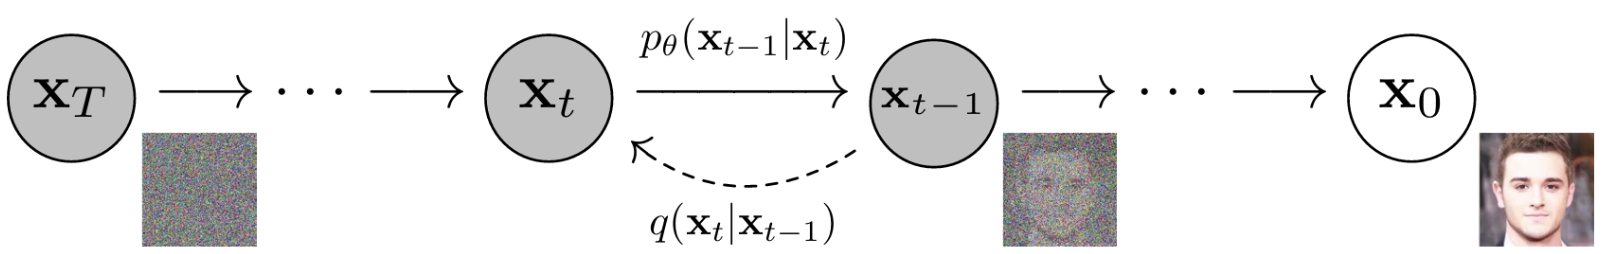
\includegraphics{figures/DiME/backward_pass_diffusion_model.png}
  \caption{Example of a forward pass (from right to left) and a
    backward pass (from left to right) in a diffusion model (from
  \cite{ho2020denoisingdiffusionprobabilisticmodels}).}
  \label{fig:backward_pass_diff_model}
\end{figure}

\paragraph{Guided diffusion}
Furthermore, this sampling procedure can be adapted to optimize
specific properties of the generated image using a scheme known as
guided diffusion \cite{dhariwal2021diffusion}. To condition the
generation on external information, such as a given label $y$, the
reverse step is shifted using the gradient of a loss function $L(x_t;
y)$ that specifies the desired property:
$$
p_\theta(x_{t-1}|x_t) = \mathcal{N}(\mu_\theta(x_t, t) -
\Sigma_\theta(x_t, t)\nabla_{x_t} L(x_t; y), \Sigma_\theta(x_t, t))
$$
This modification directly guides the denoising trajectory toward a
specific attribute, making diffusion models highly effective for
targeted image manipulations and counterfactual explanations.

\subsection{How does DiME work?}

First of all, note that DiME was introduced with different diffusion
notations. The clean image is denoted $x$ (instead of $x_0$), the
noisy image at timestep $t$ is denoted $z_t$ (instead of $x_t$), and
the cumulative product of the $1-\beta_t$ is denoted $\alpha_t$
(instead of $\bar{\alpha}_t$). To align with the DiME framework
formulation, we are going to use these notations while being careful
when dealing with previous diffusion equations.

To generate a Counterfactual Explanation, the DiME framework first
partially noises a clean image $x$ to a timestep $\tau\in\llbracket
1, T \rrbracket$ using the forward process, and then reverse the
process using guided diffusion to move the image reconstruction
towards a counterfactual, hence altered, version of the initial clean
image. The loss used during the guided diffusion is composed of a
classification term ($\mathcal{L}_\text{class}$) to guide the image
reconstruction toward the target label, and a perceptual loss
($\mathcal{L}_\text{perc}$) to ensure proximity between the former
image and its reconstruction. In the initial formulation of guided
diffusion, the classifier was trained on noisy images and thus its
gradient was informative along all the diffusion process. However,
for lack of generality and because many classifiers are only trained
over natural images, we could not extract information from the
classification loss when dealing with noisy images $z_t$. That is why
the idea of DiME is to fully reconstruct an intermediate clean image
$x_t$ (depending on $z_t$), that is used to compute clean gradients
in order to guide the diffusion of $z_t$ to $z_{t-1}$. This loop
continues until having $z_0$, the counterfactual explanation of $x$
without any remaining noise. The loss is thus expressed as:
$$
\mathcal{L}(z_t;y,x) = \mathbb{E}\left[ \lambda_c
  \mathcal{L}_\text{class}(C(y|x_t)) + \lambda_p
\mathcal{L}_\text{perc}(x_t,x) \right] = \mathbb{E}\left[
\tilde{\mathcal{L}}(x_t;y,x) \right]
$$
where $C$ is the considered classifier, $y$ is the label we want to
obtain, and thus $C(y|x_t)$ represents the posterior probability of
the category $y$ given $x_t$. Furthermore, $\lambda_c$ and
$\lambda_p$ are constants that control the trade-off between
classification guidance and perceptual proximity. It is important to
note that an expectation is taken because $x_t$ is stochastic with
respect to $z_t$. In the original DiME article
\cite{jeanneret2022diffusion}, the authors do not estimate the
expectation as an empirical mean for computational reasons, but argue
that a single realization per timestep $t$ is sufficient as it will
be averaged through the $\tau$ timesteps. Finally, they take
advantage of this source of randomness to produce diverse
counterfactual explanations from a single source image.

The $x_t$-based loss expression derives as follows:
$$\nabla_{z_t} \mathcal{L}(z_t;y,x) = \left(\frac{\partial
x_t}{\partial z_t}\right)^T \nabla_{x_t} \tilde{\mathcal{L}}(x_t;y,x)$$
where the Jacobian $\frac{\partial x_t}{\partial z_t}$ would be
computationally heavy when $t$ is high. However, we can take
advantage of the forward sampling process $z_t$ from a clean image
$x_t$, given by:
$$
z_t = \sqrt{\alpha_t}x_t + \sqrt{1-\alpha_t} \epsilon
$$
to finally have a straightforward formulation of $\frac{\partial
x_t}{\partial z_t}$ and thus derive:
$$
\nabla_{z_t} \mathcal{L}(z_t;y,x) = \frac{1}{\sqrt{\alpha_t}}
\nabla_{x_t} \tilde{\mathcal{L}}(x_t;y,x)
$$

This whole pipeline is described by \autoref{fig:DiME}.

\begin{figure}[!ht]
  \centering
  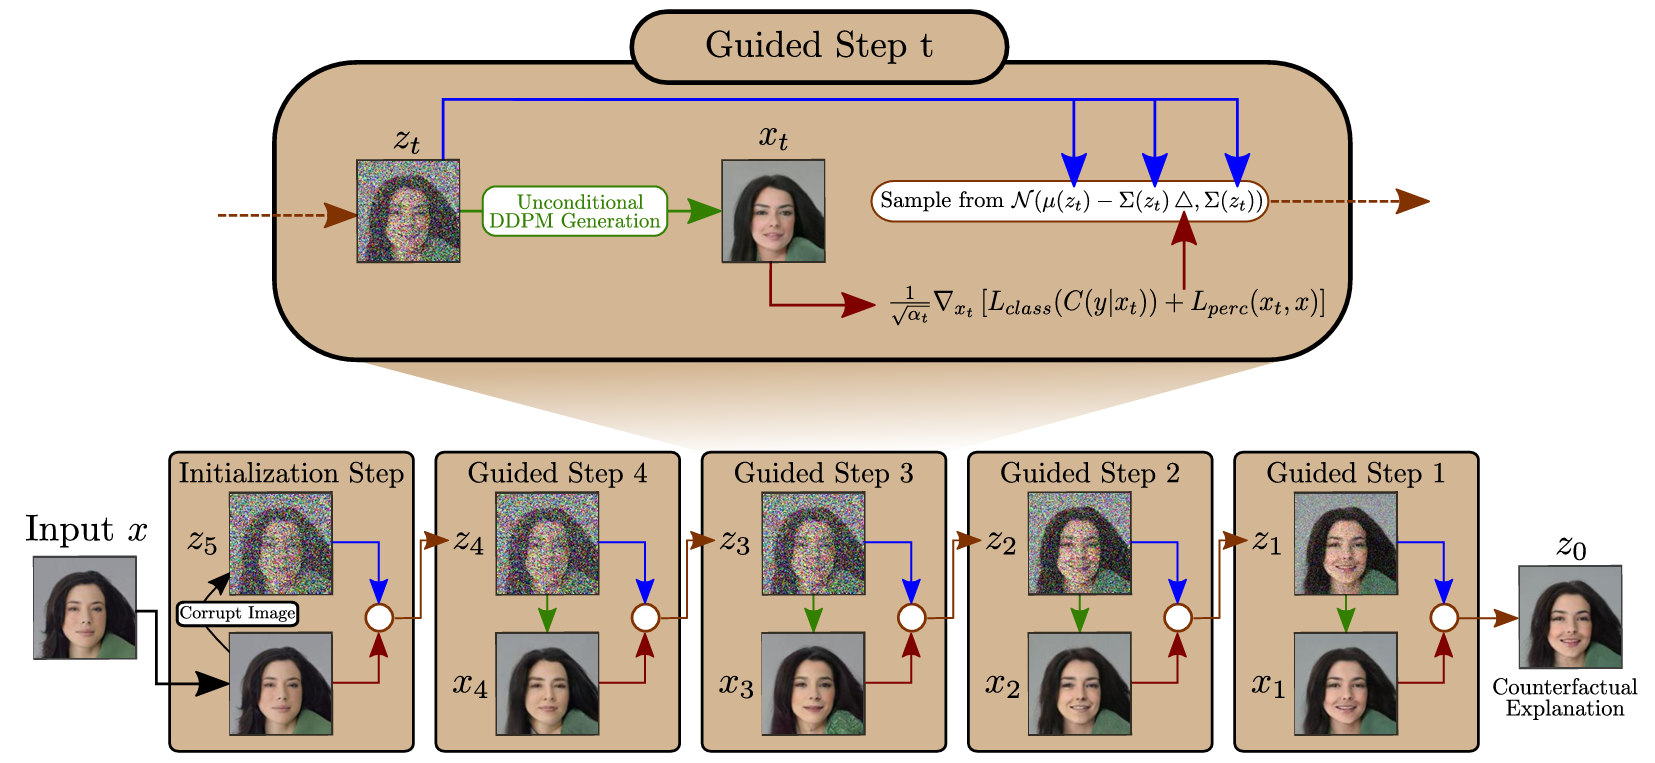
\includegraphics[width=0.9\linewidth]{figures/DiME/DiME.png}
  \caption{DiME framework scheme with $\tau=5$. At each diffusion
    step, we fully compute a clean image $x_t$ from $z_t$ using DDPM in
    order to have clean gradients to compute $z_{t-1}$ using guided
    diffusion, to have an image with lesser noise than $z_t$ and in the
  direction of being classified as $y$ by the classifier.}
  \label{fig:DiME}
\end{figure}

A final important point is that if the counterfactual clean image
$z_0$ is not classified as $y$ by the classifier, the same pipeline
is re-run with a higher $\lambda_c$ constant, to give more importance
to the class guidance in the loss expression. Finally, the method
fails if it does not find any explanation after exhausting the
provided values of $\lambda_c$.

\section{Application of DiME to audio}

This section aims to detail the implementation changes we made to
adapt the initial DiME framework, applied on natural face images, to
audio analysis, and more precisely classification from music files.

\subsection{Dataset}
The first and most important modification we propose is the data
itself. While DiME initially uses the CelebA dataset
\cite{liu2015faceattributes}, composed of human face images described
by 40 binary attributes, our implementation is based on the
OpenMIC-2018 dataset \cite{humphrey2018openmic}. It contains 20000
examples of 10-seconds music, partially labeled for the presence or
absence of 20 instrument classes by annotators on a crowd-sourcing platform.

\subsection{Data transformation}

Natural images are 2D spatial objects represented through 3 channels
(Red, Green, Blue), while a raw audio is a 1D temporal signal. To
bridge this dimensional gap, we can transform each 1D audio waveform
into its mel spectrogram, a 2D time-frequency representation that
maps the energy of the signal according to the mel scale,
approximating human pitch perception. This means that, instead of
using 3 channels images were each pixel represents a RGB color, we
are going to use 1 channel images representing magnitude of the signal.
This single-channel representation comes with an important
limitation: instrument harmonics overlap heavily in the frequency
domain, meaning guitar and piano, for instance, cannot be cleanly
separated by local edits to the spectrogram. This will inherently
limit how specific our counterfactuals can be.

\subsection{Pre-trained models}

\paragraph{DDPM}
The original DiME implementation relies on a diffusion model trained
to generate human faces, meaning its learned prior is incompatible
with our audio data. Mel spectrograms are drawn from a completely
different distribution and do not share the same features as natural
images, thus we must adapt the backbone diffusion model. We opt for
the DDPM published by Robert Dargavel Smith called
"audio-diffusion-breaks-256"\footnote{\url{https://huggingface.co/teticio/audio-diffusion-breaks-256}}
and available on hugging face. It has been trained on 30000 samples
from WhoSampled and YouTube, to generate mel spectrograms of size
256x256 corresponding to 5 seconds of audio.

\paragraph{Classifier}
Similarly, the guidance classifier $C(y|x_t)$ must be replaced to
match the new domain. We keep the original DiME DenseNet121
architecture, but trained on 5 seconds spectrograms from OpenMIC-2018
instead of face images. This network provides the posterior
probabilities for the target audio events, supplying the "clean
gradients" necessary to guide the reverse diffusion process toward
the desired audio counterfactual.

\subsection{Perceptual loss}
The perceptual loss ($\mathcal{L}_{\text{perc}}$) relies on a deep
features extractor to ensure that the counterfactual image remains
visually identifiable as the original input. In the DiME framework,
the authors naturally used the standard VGG19 perceptual loss
extracting visual features from the images. However, maintaining the
visual similarity of spectrograms based on a natural image feature
extractor does not strictly guarantee audio similarity. For this
reason, we used the Pretrained Audio Neural Networks (PANNs) CNN-14,
a feature extractor built specifically for handling spectrograms.
However, CNN14 was designed for audio tagging, not similarity
measurement. Its features encode semantic content rather than
fine-grained acoustic texture. The perceptual term may end up
competing with the classification guidance rather than complementing
it. A contrastive audio encoder could have been better suited here.

\subsection{Metrics}
\label{sec:metrics}
Evaluating the realism and quality of the generated counterfactuals
requires domain-appropriate metrics. While the original paper uses
the Fréchet Inception Distance (FID) to measure image fidelity
against the CelebA distribution, our audio implementation relies on
the Fréchet Audio Distance (FAD). Instead of using visual embeddings,
FAD utilizes audio embeddings (typically extracted via a pre-trained
VGGish model) to compare the continuous distribution of the real
audios from the dataset against our generated counterfactual
spectrograms, providing a robust measure of acoustic plausibility.
Finally, note that the counterfactual explanation of audio, and more
precisely of music, has not been widely studied yet, so we cannot
compare our results with other articles.

In addition to FAD, we report metrics that quantify (i) whether the
desired classification change is achieved, and (ii) how strongly the
counterfactual deviates from the original sample. Let $x^{(i)}$ be the
original mel-spectrogram (treated as an image-like tensor), $\tilde{x}^{(i)}$
its counterfactual, $w^{(i)}$ and $\tilde{w}^{(i)}$ the corresponding
time-domain waveforms, and $p^{(i)}_k$ (resp.\ $\tilde{p}^{(i)}_k$) the
classifier posterior probability for class $k$ before (resp.\ after).
We denote by $y$ the target class and by $p$ the decision threshold
(we use $p=0.5$). All reported values are averaged over $N$ samples.

\paragraph{Flip ratio (\%).}
This measures the fraction of samples for which the classifier decision
for the \emph{target} class changes between the original and the
counterfactual:
$
\mathrm{Flip}(\%) \;=\;
100 \cdot \frac{1}{N}\sum_{i=1}^{N}\mathbf{1}\!\left[
  \mathbf{1}\!\left(p^{(i)}_{y}> p \right)\neq
  \mathbf{1}\!\left(\tilde p^{(i)}_{y}> p \right)
\right].
$
A high flip ratio indicates that counterfactuals achieve the intended
class change.

\paragraph{$\ell_1$ proximity (L1 Prox).}
We quantify how close the counterfactual spectrogram remains to the
original in pixel space:
$
\mathrm{L1\ Prox} \;=\; \frac{1}{N}\sum_{i=1}^{N}\left\lVert
\tilde{x}^{(i)} - x^{(i)} \right\rVert_{1}$.

\paragraph{MNAC (Mean Number of Attributes Changed).}
Because our classifier is multi-label, it is important to check whether
non-target instruments are unintentionally modified. MNAC counts how many
\emph{non-target} labels change their binary decision after thresholding:
$
\mathrm{MNAC} \;=\;
\frac{1}{N}\sum_{i=1}^{N}\;\sum_{k\neq y}
\mathbf{1}\!\left[
  \mathbf{1}\!\left(p^{(i)}_{k}> p \right)\neq
  \mathbf{1}\!\left(\tilde p^{(i)}_{k}> p \right)
\right].
$
Lower MNAC means more class-specific counterfactual changes.

\paragraph{SNR (dB).}
In the time domain, we measure a signal-to-noise ratio between the
original waveform and the counterfactual:
$
\mathrm{SNR(dB)} \;=\;
10\log_{10}\!\left(
  \frac{\frac{1}{T}\sum_{t=1}^{T}\left(w^{(i)}_t\right)^2+\varepsilon}
  {\frac{1}{T}\sum_{t=1}^{T}\left(\tilde
  w^{(i)}_t-w^{(i)}_t\right)^2+\varepsilon}
\right),
$
with a small constant $\varepsilon>0$ for numerical stability. Higher
SNR indicates stronger waveform preservation.

\paragraph{LSD (Log-Spectral Distance).}
We also report a spectral distortion measure based on STFT magnitudes.
Let $S_w(f,m)$ denote the STFT magnitude at frequency bin $f$ and time
frame $m$. Then:
$
\mathrm{LSD} \;=\;
\frac{1}{M}\sum_{m=1}^{M}\sqrt{\frac{1}{F}\sum_{f=1}^{F}\left(
    20\log_{10}\!\left(\left|S_{w}(f,m)\right|+\varepsilon\right)
    -
    20\log_{10}\!\left(\left|S_{\tilde w}(f,m)\right|+\varepsilon\right)
\right)^{2}}.
$
Lower LSD indicates closer spectra.

\paragraph{Mean cosine similarity (embedding-based source preservation).}
To better reflect perceptual similarity beyond sample-wise distances,
we compute the cosine similarity between embeddings extracted from a
pre-trained audio network $f(\cdot)$:
$
\mathrm{CosineSim} \;=\;
\frac{1}{N}\sum_{i=1}^{N}
\frac{\left\langle f(w^{(i)}),\,f(\tilde w^{(i)})\right\rangle}
{\left\lVert f(w^{(i)})\right\rVert_{2}\;\left\lVert f(\tilde
w^{(i)})\right\rVert_{2}}.
$
Higher values indicate better preservation of the original content in
the embedding space.

\paragraph{FAD (Fréchet Audio Distance).}
Finally, we compute FAD by comparing the distribution of embeddings of
reference audios and counterfactual audios. If $(\mu,\Sigma)$ and
$(\tilde\mu,\tilde\Sigma)$ are the empirical mean and covariance of the
reference and counterfactual embedding sets, respectively, then:
$
\mathrm{FAD} \;=\;
\left\lVert \mu - \tilde\mu \right\rVert_{2}^{2}
\;+\;
\mathrm{Tr}\!\left(\Sigma+\tilde\Sigma-2\left(\Sigma\tilde\Sigma\right)^{1/2}\right).
$
Lower FAD indicates that counterfactuals are closer to the reference
audio distribution in the chosen embedding space (e.g.\ VGGish).
%

\subsection{Overview of our experiment}

\begin{figure}
  \centering
  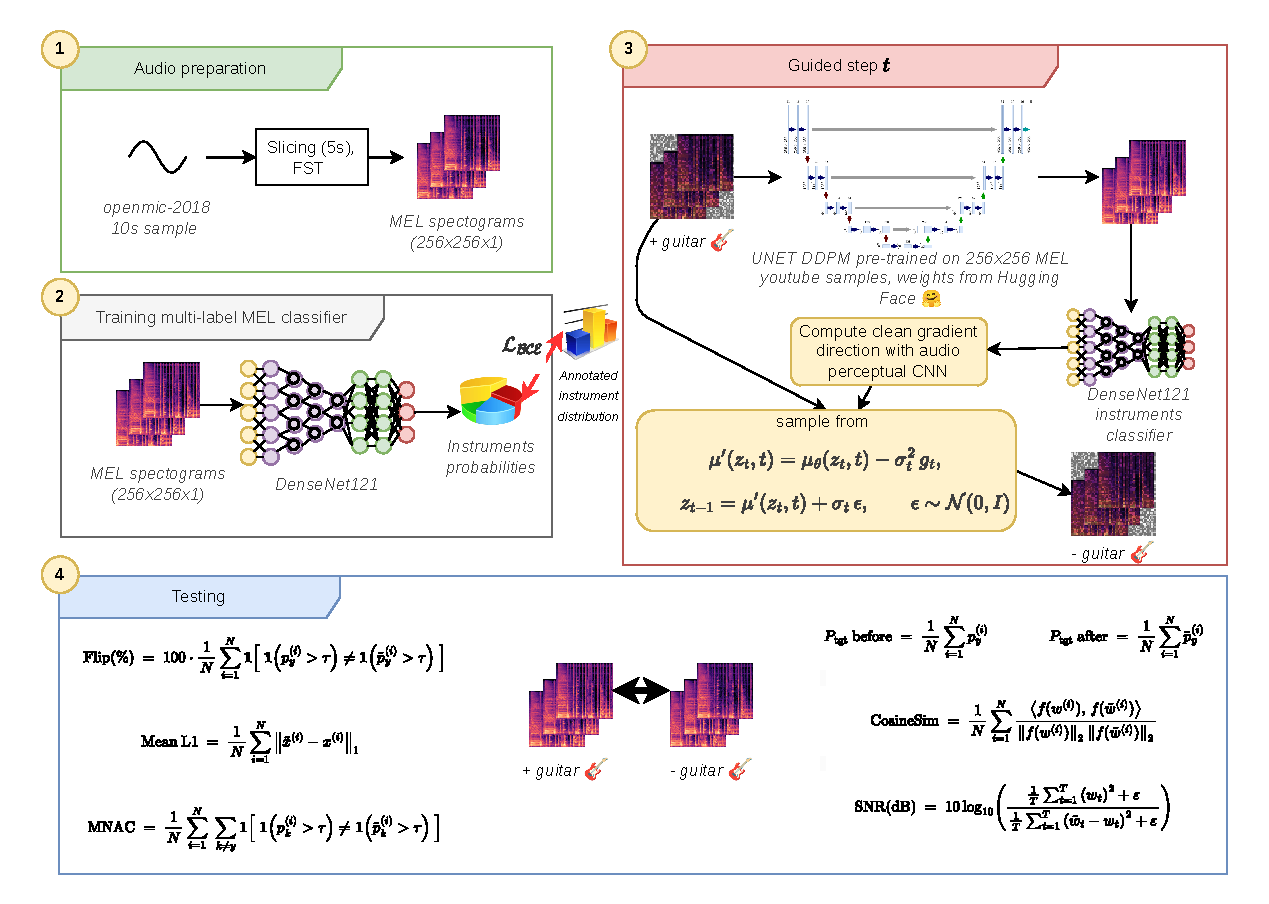
\includegraphics[width=0.9\linewidth]{figures/experiments-setup.pdf}
  \caption{Scheme of our audio adaptation of the DiME framework. The
    main differences with the original DiME are the data (from face
    images to music spectrograms), the pre-trained models (from a
      DDPM trained on faces and a classifier trained on CelebA to a
    DDPM trained on spectrograms and a classifier trained on OpenMIC),
    and the perceptual loss (from VGG19-based to CNN14-based). First,
    we transform the audio samples to MEL spectrograms of 5seconds
    (openmic-2018 samples), then we train a classifier on these
    spectograms to predict the presence of the 20 instruments. Finally,
    we use the pre-trained DDPM to generate counterfactual spectrograms
    with the DiME pipeline, and we evaluate them using the metrics
  described in \autoref{sec:metrics} }
  \label{fig:DiME_audio}
\end{figure}

\section{Results}

Given an input spectrogram $x$, we sample a
partially noised
version $z_{\tau}\sim q(z_\tau\mid x)$ at timestep $\tau=160$ and run
the reverse
diffusion process to obtain a counterfactual $\tilde{x}$.
Guidance is computed from the multi-label DenseNet121 classifier
together with proximity regularization, combining an $\ell_1$ term (weight
$\lambda_{\ell_1}=0.02$) and a CNN14-based perceptual term (weight
$\lambda_p=20$).
For classifier guidance, we use a scale $\lambda_c=100$.

Our experiment task is to remove the electric guitar (and other instruments such
as drums) from the input spectrogram,
(the \texttt{guitar\_removal\_hq} run), targets are specified
explicitly: we provide a sequence of target class indices with
\texttt{--target\_labels} and set the desired direction to removal
($y_{\mathrm{val}}=0$),
producing sequential counterfactual steps saved as \texttt{step\_0},
\texttt{step\_1}.
We apply guidance only during the first 20 reverse steps (parameter
\texttt{guided\_iterations}=20); the remaining denoising steps follow
the unguided
reverse diffusion dynamics.

\subsection{Qualitative results}

We first provide qualitative evidence that the proposed guided diffusion
procedure can produce counterfactual mel-spectrograms that remain close to the
input while introducing structured, localized changes.
\autoref{fig:qualitative_step0} shows (i) the original spectrogram, (ii) the
generated counterfactual at Step~0, and (iii) an absolute difference map.
The difference map suggests that the edit is not a global corruption of the
spectrogram, but rather a sparse modification pattern, which is consistent with
the relatively small $\ell_1$ proximity values reported in
\autoref{tab:main_results}.

\begin{figure}[!ht]
  \centering
  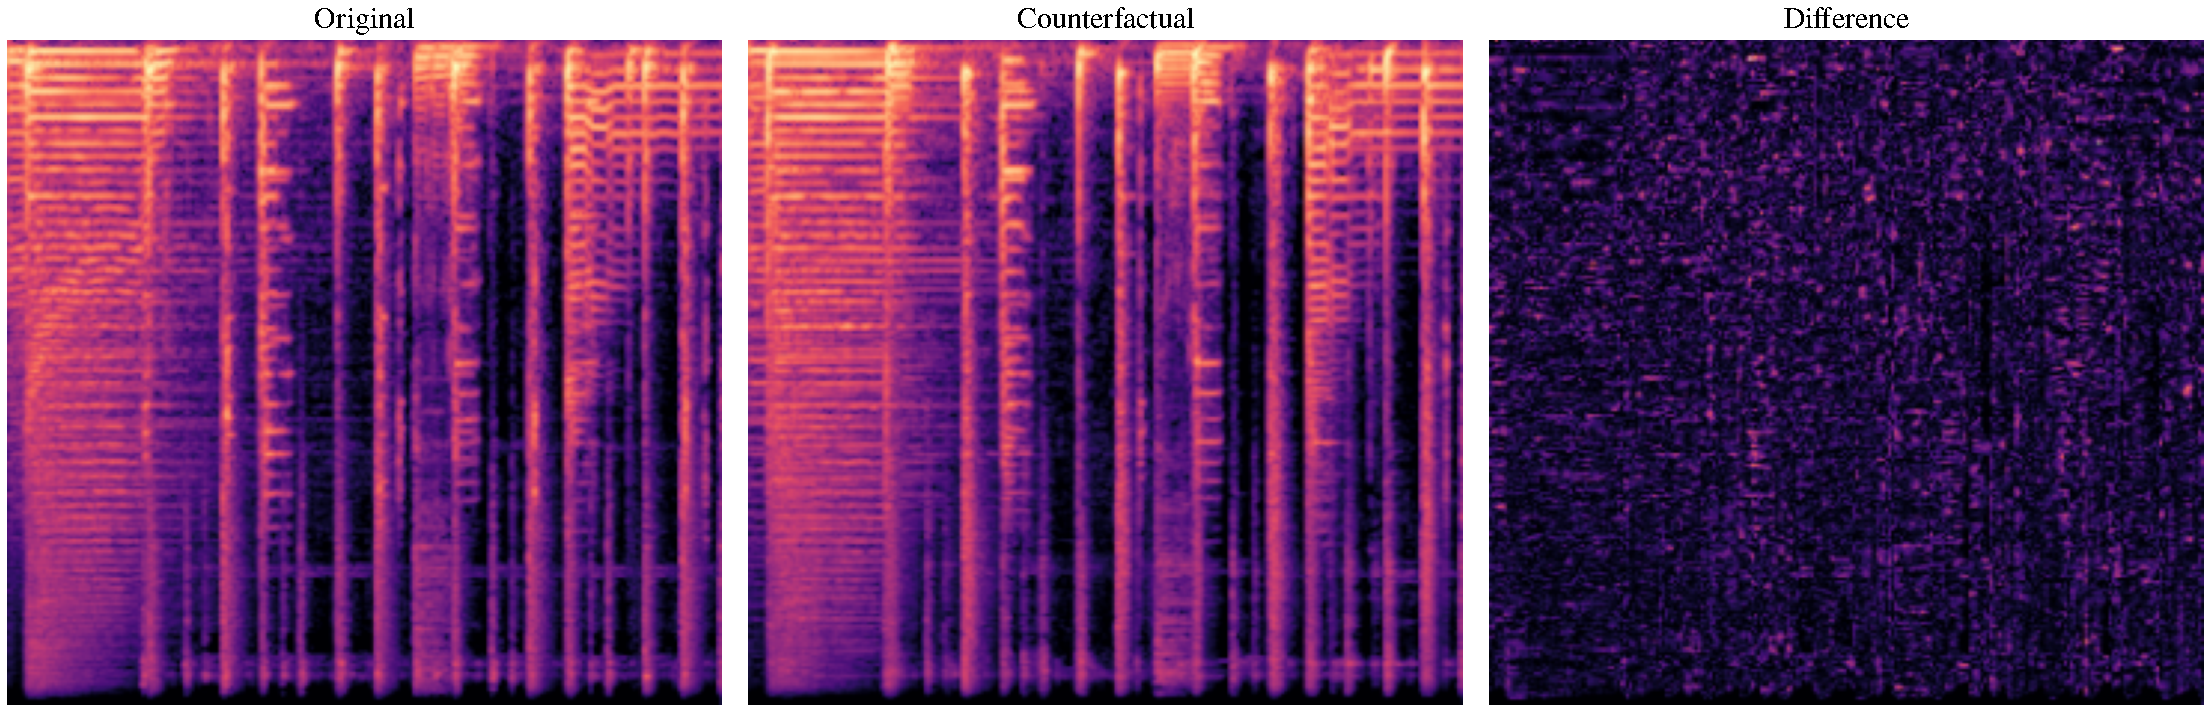
\includegraphics[width=0.95\linewidth]{figures/guitar_removal_hq_step0_sample0_comparison.pdf}
  \caption{Qualitative comparison (\texttt{guitar\_removal\_hq},
    Step~0, sample~0):
    original mel-spectrogram (left), counterfactual (middle), and absolute
  difference map (right).}
  \label{fig:qualitative_step0}
\end{figure}

We also listen to the reconstructed waveforms corresponding to the original and
counterfactual spectrograms. The original sample contains a electric
guitar, while the
counterfactual is intended to remove it. Subjectively, we can confirm that the
electric guitar and drums are less audible in the counterfactual,
while other instruments
are still present. The samples are available here\footnote{original:
\url{https://github.com/aygoun/mva-DiME/raw/refs/heads/main/audio/results/guitar_removal_hq/step_0/original_wav/000000.wav}}\footnote{counterfactual
  at step 5 (after electric guitar removal):
\url{https://github.com/aygoun/mva-DiME/raw/refs/heads/main/audio/results/guitar_removal_hq/step_5/cf_wav/000000.wav}}.
In the counterfactual sample, the electric guitar "looks like" more a
synthesizer / piano sound.
Our result are not perfect, this could come from the perceptual loss
not being perfectly adapted to the audio domain, as we reused a
pre-trained model.
Note that a step correspond to a class flip, so \texttt{step\_0} is
the original sample and the first counterfactual, and
\texttt{step\_5} is the final counterfactual
after 5 flips (removing electric guitar, drums, etc.).

\subsection{Quantitative results}

We report quantitative results for the sequential counterfactual experiment
\texttt{guitar\_removal\_hq}. \autoref{tab:main_results} summarizes the main
metrics per step (flip ratio, proximity, and waveform-based similarity). In
addition, \autoref{tab:target_conf} reports target confidence statistics before
and after the edit.

\begin{table}[H]
  \centering
  \caption{Main quantitative results for \texttt{guitar\_removal\_hq}.
    Flip Ratio measures success for the target edit; L1 Prox measures
    spectrogram proximity; MNAC counts non-target label changes.
  SNR and LSD are computed on reconstructed waveforms.}
  \label{tab:main_results}
  \begin{tabular}{llrrrrr}
\toprule
 &  & Flip Ratio (\%) & L1 Prox & MNAC & SNR (dB) & LSD \\
experiment & step &  &  &  &  &  \\
\midrule
\multirow[t]{6}{*}{guitar\_removal\_hq} & 0 & 100.000000 & 0.110702 & 1.800000 & -2.950137 & 9.364269 \\
 & 1 & 62.500000 & 0.106687 & 3.000000 & -3.073757 & 9.210129 \\
 & 2 & 100.000000 & 0.107320 & 2.375000 & -2.981012 & 9.261023 \\
 & 3 & 100.000000 & 0.106692 & 2.125000 & -2.908162 & 9.258429 \\
 & 4 & 100.000000 & 0.105072 & 1.875000 & -3.239836 & 9.221994 \\
 & 5 & 100.000000 & 0.104598 & 1.375000 & -3.153058 & 9.172865 \\
\cline{1-7}
\bottomrule
\end{tabular}

\end{table}

\begin{table}[H]
  \centering
  \caption{Per-step target-class evaluation for \texttt{guitar\_removal\_hq}.
    $P_{\mathrm{tgt}}$ denotes the classifier posterior probability
    for the target
  class before and after counterfactual generation.}
  \label{tab:target_conf}
  % eval\_metrics\_v2: experiment guitar\_removal\_hq (generated file)
\begin{tabular}{crrrrrr}
\hline
Step & Samples & Flip (\%) & Mean L1 & MNAC & $P_{\mathrm{tgt}}$ before & $P_{\mathrm{tgt}}$ after \\
\hline
0 & 10 & 100.00 & 0.110702 & 1.8000 & 0.1670 & 0.0996 \\
1 & 8 & 62.50 & 0.106687 & 3.0000 & 0.8218 & 0.3656 \\
2 & 8 & 100.00 & 0.107320 & 2.3750 & 0.6552 & 0.0963 \\
3 & 8 & 100.00 & 0.106692 & 2.1250 & 0.6480 & 0.1863 \\
4 & 8 & 100.00 & 0.105072 & 1.8750 & 0.3103 & 0.0619 \\
5 & 8 & 100.00 & 0.104598 & 1.3750 & 0.5214 & 0.1049 \\
\hline
\end{tabular}

\end{table}

Overall, flip ratios are high across steps (often reaching $100\%$), showing
that classifier guidance effectively enforces the requested edit.
Step~1 is more challenging (flip ratio $62.5\%$) and also exhibits the largest
MNAC, suggesting that achieving the target flip at that stage may induce more
side effects on other predicted instruments.
Across steps, the mean $\ell_1$ proximity remains relatively stable (around
$0.10$--$0.11$), indicating that counterfactuals remain close in spectrogram
space.

Waveform-based distortion metrics (SNR, LSD) are substantially degraded.
In our setting, these metrics depend on the spectrogram-to-audio inversion
procedure (used to reconstruct waveforms), which can introduce artifacts.
We therefore also report embedding-based similarity and distributional metrics
computed directly on available waveform pairs.

\begin{table}[!ht]
  \centering
  \caption{Embedding-based similarity and realism metrics computed on waveform
    pairs available for evaluation. Cosine similarity is computed between
    embeddings of original and counterfactual waveforms. FAD compares the
  embedding distributions of original vs. counterfactual audio.}
  \label{tab:audio_embedding_metrics}
  % evaluate\_similarity: original\_wav\_\_cf\_wav (generated)
\begin{tabularx}{\textwidth}{lcc}
  \hline
  Pairs & Mean cosine similarity & Embedding model \\
  \hline
  8 & 0.9772 & microsoft/unispeech-sat-base-plus-sv \\
  \hline
\end{tabularx}

  \vspace{0.5em}
  % evaluate\_fad: original\_wav\_\_cf\_wav (generated)
\begin{tabularx}{\textwidth}{lc}
  \hline
  Embedding model & FAD \\
  \hline
  vggish & 2.7064 \\
  \hline
\end{tabularx}

\end{table}

\subsection{Discussion}

The quantitative results confirm the intended behavior of our guided diffusion
pipeline: the target confidence $P_{\mathrm{tgt}}$ consistently decreases after
counterfactual generation when performing a removal edit, and the flip ratio is
high for most steps (\autoref{tab:target_conf}). At the same time, MNAC shows
that non-target predictions can change as a side effect, especially in the most
difficult steps (e.g., Step~1). This reflects the inherent entanglement of
instrument cues in music spectrograms and the fact that classifier gradients are
not guaranteed to be class-disentangled.

From a fidelity perspective, the relatively small L1 proximity values suggest
that edits remain limited in spectrogram space (\autoref{tab:main_results}), and
the embedding cosine similarity remains high
(\autoref{tab:audio_embedding_metrics}), indicating that much of the global
audio content is preserved in a learned audio representation.

Finally, the discrepancy between spectrogram-space proximity and waveform-based
distortion metrics suggests that waveform reconstruction can be a bottleneck for
audio evaluation in our setting. This motivates the use of embedding-based
metrics (similarity, FAD) and points toward future improvements such as
better inversion/vocoder components or end-to-end evaluation directly in the
spectrogram domain.

\section{Limitations and difficulties}

Initially, the goal of this project was to reimplement a portion of
DiME, as its code is not explicitly linked in the paper and the
instruction given in the list of papers was not about changing the
modality. However, after further research, we found the paper's
official GitHub
repository\footnote{\url{https://github.com/guillaumejs2403/DiME}}
containing the complete implementation. Thus, we decided to change
our approach and apply the framework to a completely new modality
that is the audio.

The primary challenge we encountered was not the structural shift to
2D audio representations, but rather the lack of available
pre-trained models for our target domain. Initially, we wanted to
adapt DiME to the FSD50K dataset \cite{fonseca2022FSD50K}, composed
of diverse environmental sound events annotated with 200 binary
attributes such as "Male speech" or "Wind". However, we were
constrained by the absence of a robust and open-source DDPM trained
on general background noise, and training our own was out of the
scope of this project. Because the only suitable pre-trained
diffusion model we found was trained specifically on music
spectrograms, we finally adapted our pipeline from general sound
classification to music-specific tasks. Furthermore, we could not
find a suitable pre-trained classifier on this new domain, so we
ended-up by training our own from scratch. Because other audio
results do not exist it is hard to compare them, but we can think
that combining a niche DDPM with a custom classifier led to poorer
results than the original DiME framework, based on state-of-the-art
models in the heavily studied area that is the face analysis.
Finally, due to computational constraints, we were only able to
evaluate on 8-10 samples per step, which is insufficient to draw
statistically meaningful conclusions from the reported metrics.

\newpage
\printbibliography

\end{document}
